
\centerline{\textbf{ \LARGE Data Path }}

\begin{questyle}
  \question  Consider the following data path of a simple non-pilelined CPU. The registers A, B, A1, A2, MDR,
             the bus and the ALU are 8-bit wide. SP and MAR are 16-bit registers. The MUX is of
             size 8 × (2:1) and the DEMUX is of size 8 × (1:2). Each memory operation takes 2 CPU
             clock cycles and uses MAR (Memory Address Register) and MDR (Memory Date Register).
             SP can be decremented locally. How many CPU clock cycles are needed to execute the
             "push r" instruction? The CPU instruction \mbox{"push r"}, where = A or B, has
             following specification. (GATE-2001) \\ M[SP]\(\leftarrow\)r \\ SP\(\leftarrow\)(SP – 1)

             \begin{myTableStyle} \begin{tabular}{ |m{14cm}| } \hline
                  \begin{center} 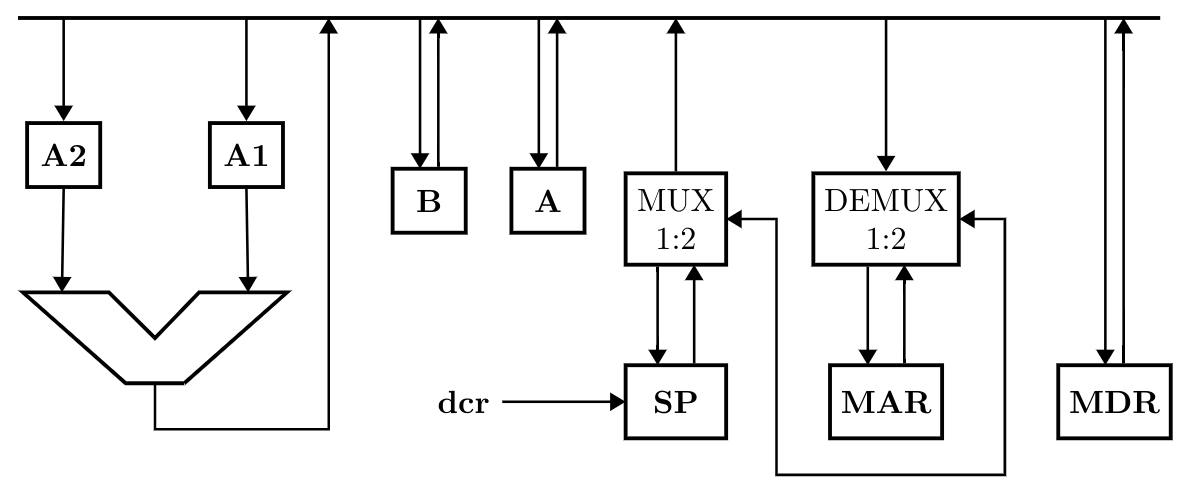
\includegraphics[scale=0.3]{./images/data_path_01.png} \end{center}\\ \hline
            \end{tabular} \end{myTableStyle} \vspace{0.08in}

  \begin{oneparchoices}
    \choice         2
    \choice         3
    \choice         4
    \CorrectChoice  5
  \end{oneparchoices}
  \\ Hint: \qquad CPU has to fill MAR and MDR before memory operation takes place.
  \\ Hint: \qquad 2-cycles \qquad \qquad MAR(2 Byte) \(\leftarrow\) SP(2 Byte) \quad using 8-bit bus
  \\ Hint: \qquad 1-cycles \qquad \qquad MDR(1 Byte) \(\leftarrow\) A(1 Byte) \quad using 8-bit bus
  \\ Hint: \qquad 2-cycles \qquad \qquad Memory Operation
\end{questyle}

\begin{questyle}
  \question  Consider the following sequence of micro-operations. Which one of the following
            is a possible operation performed by this sequence?  (GATE-2013)
            \\ \qquad MBR\(\leftarrow\)PC
            \\ \qquad MAR\(\leftarrow\)X
            \\ \qquad PC\(\leftarrow\)Y
            \\ \qquad Memory\(\leftarrow\)MBR \\
  \begin{oneparchoices}
    \choice         Instruction fetch
    \choice         Operand fetch
    \choice         Conditional branch
    \CorrectChoice  Initiation of interrupt service
  \end{oneparchoices}
\end{questyle}

\begin{questyle}
  \question  Consider the following data path of a CPU. The, ALU, the bus and all the registers
             in the data path are of identical size. All operations including incrementation of the
             PC and the GPRs are to be carried out in the ALU. Two clock cycles are needed for
             memory read operation - the first one for loading address in the MAR and the next
             one for loading data from the memory bus into the MDR. (GATE-2005)

             \begin{myTableStyle} \begin{tabular}{ |m{14cm}| } \hline
                  \begin{center} 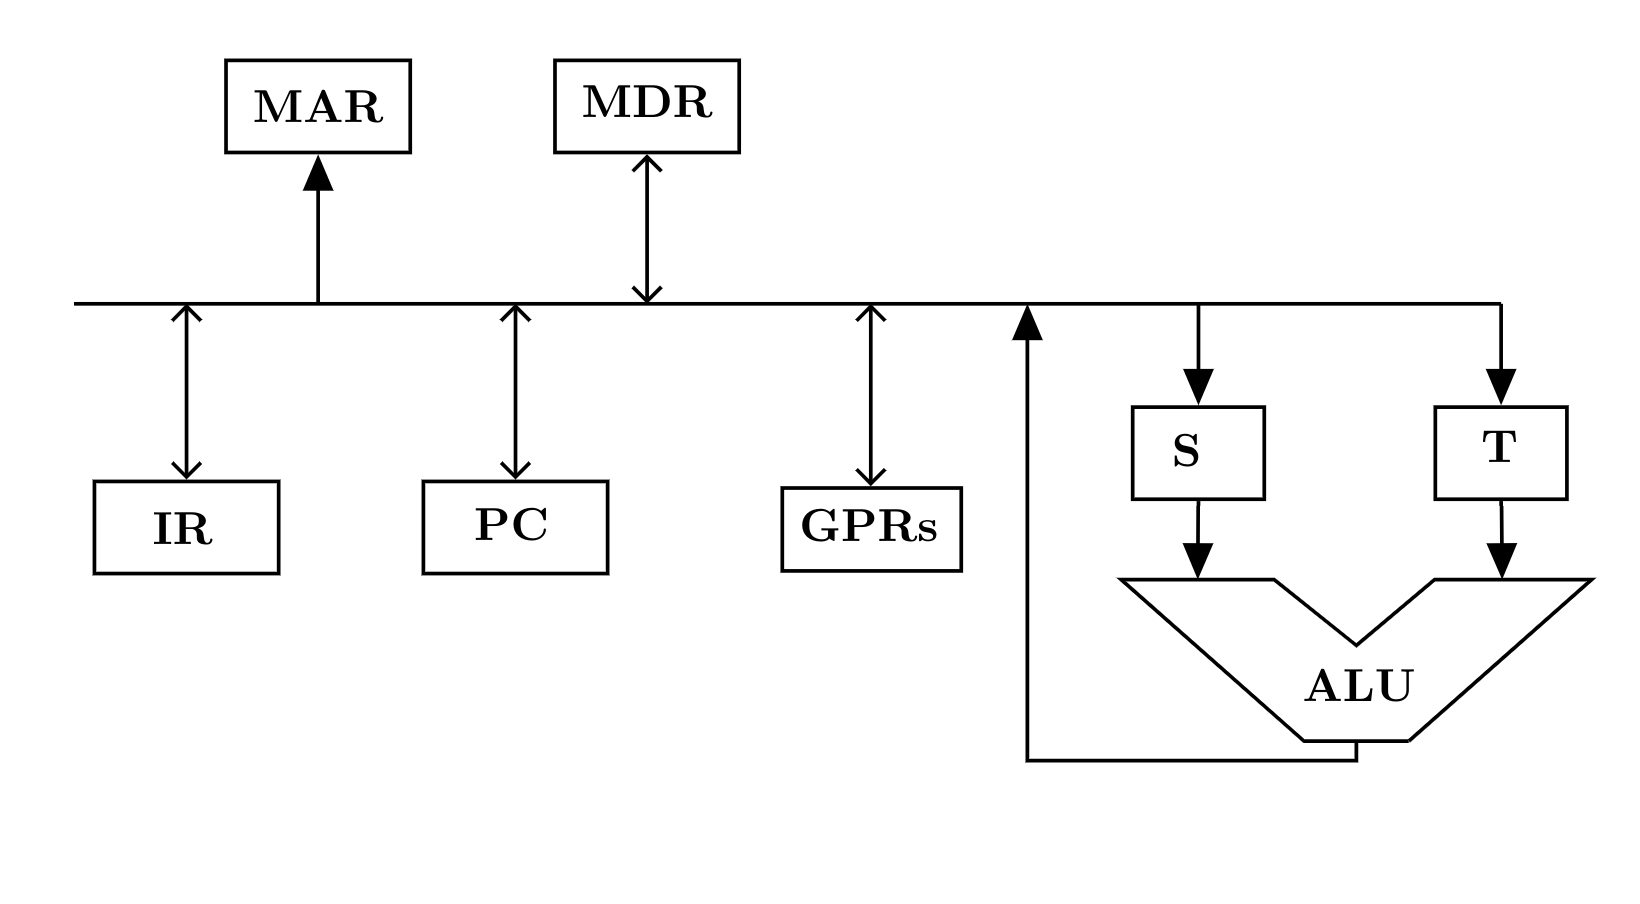
\includegraphics[scale=0.15]{./images/data_path_02.jpeg} \end{center}\\ \hline
            \end{tabular} \end{myTableStyle} \vspace{0.08in}

             \begin{parts}
             \part The instruction "ADD R0, R1" has the register transfer interpretation R0\(\leftarrow\)R0 + R1
                   The minimum number of clock cycles needed for execution cycle of this instruction is:
              \begin{oneparchoices}
                \choice         2
                \CorrectChoice  3
                \choice         4
                \choice         5
              \end{oneparchoices}
              \\ Hint : 1st cycle : S\(\leftarrow\)R0
              \\ Hint : 2nd cycle : T\(\leftarrow\)R1
              \\ Hint : 3rd cycle : ALU operation and R0{ \Large \( \leftarrow ALU_{result}  \) }

             \part The instruction "call Rn, sub" is a two word instruction.  The minimum number of clock
                   cycles needed for execution cycle of this instruction is? Assuming that PC is
                   incremented during the fetch cycle of the first word of the instruction, its
                   register transfer interpretation is.
                   \\ \qquad Rn \(\leftarrow\) PC + 1; \\ \qquad PC \(\leftarrow\) M[PC]; \\
            \begin{oneparchoices}
              \choice         2
              \CorrectChoice  3
              \choice         4
              \choice         5
            \end{oneparchoices}
              \\ Hint : 1st cycle : [S, MAR]\(\leftarrow\)PC
              \\ Hint : 2nd cycle : MDR\(\leftarrow\)Memory \qquad ALU operation: Rn{ \Large \( \leftarrow ALU_{result}(S+1)  \) }
              \\ Hint : 3rd cycle : PC\( \leftarrow\)MDR

             \end{parts}
\end{questyle}
